\chapter{Overview}\label{ch:Meat}

\section{Description of Problem}
As part of my MSc thesis, I studied in detail the OCS Van der Waals (VdW) dimer. Although interesting by itself, one of the main goals of that work was to test 
current electronic ab initio methods on a tough system. VdW complexes are perfect for this because of 
their wide range of motion and numerous minima. These calculations demonstrated that the current ab 
initio methods used to generate a Potential Energy Surface (PES) are very accurate. 

I would like to test the accuracy of a PES composed of OCS-OCS pair-wise interactions when applied to 
the OCS trimer. It may seem like a small step to calculate the rovibrational energies of the 
OCS trimer after successfully calculating the rovibrational energies of
the OCS dimer, however, it is a significant leap in
terms of complexity. Using the product basis given in Eq.~(\ref{eq.product}), the number of basis functions increases exponential with dimensionality. Dimer to trimer will increase the  
dimensionality of the system from 4D to 9D. The $J=0$ basis functions used in my previous work of 
Ref.~\citenum{Brown2012} would cause the matrix representation to be intractable. Quantifying this intractability 
using memory, the RAM required to store one double precision dimer vector (for the Lanczos iterations) 
is 61 megabytes, while the trimer vector would require well over a terabyte. This is computational 
infeasible, and necessitates a development that will drastically reduce the number of basis functions.

I plan to do this by using basis functions that are localized in the various minima 
instead of across the whole coordinate space. The hypothesis is that having basis functions with 
significant amplitude where the wavefunction is very small is superfluous. The rovibrational calculation in Ref.~\citenum{Brown2012} was performed using general polar coordinates.  The one dimensional basis functions used for the $\theta$ coordinates, for the product basis, are largely composed from legendre polynomials.  A few of these are shown in Figure \ref{fig.ass}.  Clearly, these functions are localized across the entire range of $\theta$ whereas the minima are not.
\begin{figure}[!ht]
\begin{center}
\includegraphics[scale=0.9]{associated.eps}
\caption{Associated Legendre Polynomials for $m=0$.}
\label{fig.ass}
\end{center}
\end{figure}

\section{Review of methods with localized basis functions}
 There are two methods 
currently being developed to reduce the number of basis functions by using localized functions. The first is the 
Distributed Gaussian Basis (DBG)\cite{Hamilton1986}, while the second is the phase space\cite{Davis1979} approach. Both have been 
applied to simple 1D systems (like the Morse potential), while DGB has calculated the vibration (without 
rotation) of H$_2$O and the neon/argon trimer\cite{Garashchuk2001}. 

\subsection{Distributed Gaussian Basis}
The basic premise of the DGB method is to place a bunch of Gaussian functions where the potential is lowest.  Gaussian functions have the property that they are localized in both  coordinate and momentum space.  

\subsubsection{Basis Functions}
The basis functions used for DGB are of the form\cite{Hamilton1986}
\begin{equation}
\label{eq.p1}
\phi_i=\left(\dfrac{2 A_i}{\pi}\right)^{(1/4)}\exp\left[-A_i\left(x-x_i\right)^2\right]
\end{equation}
where $A_i$ is the width parameter of a Gaussian function located at $x_i$. Since a set of Gaussian functions is not orthogonal, the use of the FBR  will require one to solve a generalized eigenvalue problem of the form
\begin{equation}
Hu=SEu
\end{equation}
where $H$ is the Hamiltonian you are solving and $S$ is the overlap matrix.  Both $H$ and $S$ are real symmetric matrices. Generally, the Hamiltonian can be decomposed into a kinetic energy portion $K$ and the potential (PES) $V$.  This results in,
\begin{equation}
\label{eq.p2}
\left(K+V\right)\phi = S\phi
\end{equation}
where for the matrix K, the integrals are evaluated exactly, while the potential integrals are most commonly evaluated using quadrature.  If the Watson Hamiltonian\cite{Watson1968} is used with a potential in Taylor expanded form, the matrix elements can be evaluated analytically. However, there is not a huge advantage to producing the $V$ matrix analytically since the product of two exponentials is also an exponential. So integrals can be performed with few gauss-quadrature points.  
This basis has a trade off between using large and small $A_i$.  A small $A_i$ leads to large kinetic energy matrix elements but lower conditions numbers.  Large $A_i$ leads to smaller kinetic energy matrix elements but large condition numbers in the matrix\cite{Garashchuk2001}. In the original outline of the Method in Ref. \citenum{Hamilton1986}, two choices of the centres $x_i$ for the DGB were given.  The first was equal spacing and the second using a semi-classical approximation. 



\subsubsection{Choosing the points}
Choosing the points semi-classically begins by noting that the $n$th exact bound state wave function has $n-1$ nodes.  When you look at the system semi-classically, the distance between two points $x_i$ and $x_{i+1}$ is,
\begin{equation}
\label{eq.b3}
\Delta J_n=\int_{x_i}^{x_{i+1}}p\left(x\right)dx,
\end{equation}
where $p\left(x\right)$ is the classical momentum $\sqrt{2m\left(E_n-V\left(x\right)\right)}$. Once you choose an energy $E_n$, you can determine the classical turning points $x_{min}$ and $x_{max}$. The number of levels at energy at or below $E_n$ labelled $R_L=n+1$ can be defined as
 \begin{equation}
\label{eq.b5}
R_l=\dfrac{1}{\pi}
\int^{x_{max}}_{x_{min}}p\left(x\right) dx+1/2 =M+1. 
 \end{equation}
This is a fairly accurate equation for quantum problems, $E_{23}$ of the Morse potential defined in Ref. \citenum{Hamilton1986} was found to have an $R_L$ value of $24$.  If you happen to want one Gaussian between each node, then the points can be found using,
\begin{equation}
\label{eq.pg}
\int^{x_1}_{x_{min}}p\left(x\right) dx =\pi/4; \quad
 \int^{x_i}_{x_{i-1}}p\left(x\right) dx =\pi
 \end{equation}
where $x_{min}$ is the classical turning point. 
 
 
If greater or fewer points are wanted, the transformation 
 \begin{equation}
\label{eq.b6}
\pi \rightarrow \pi\dfrac{R_l-1/2}{M-1/2}
 \end{equation}  
 results in the appropriate semiclassical spacing using Eq.~(\ref{eq.pg}) with the $M$ desired basis functions.  The next set of parameters that need to be chosen is the DGB widths $A_i$.  In Ref. \citenum{Hamilton1986}, the widths were chosen as
\begin{equation}\label{eq.ai}
A_1=c^2/\left(x_2-x_1\right)^2,\;A_i=4c^2/\left(x_{i+1}-x_{i-1}\right)^2,\;A_N=c^2/\left(x_N-x_{N-1}\right)^2
\end{equation}
where $c$ is a free parameter that is chosen depending on the system analysed.  The reasoning for the dependence on the distance between nearby functions was to ensure that the $A_i$ values remained large enough as to not cause the basis functions to be linearly dependant.  The justification for the $1/\left(x_{i+1}-x_{i}\right)^2$ dependence comes from analysis of the overlap matrix $S$. It's found that in the large $M$ limit, the $S$ matrix becomes diagonal insinuating that the DGB becomes a series of $\delta$ functions, or not formally overcomplete.  Overcompleteness results in many eigenvalues near zero and numerically instability (large condition number).  Interestingly, even with the $S$  matrix having a condition number on the order of $10^{10}$, the precision of the computed eigenvalues is not effected until about the 10th digit.

This choice of basis functions does not generalize well to higher dimensions.  In a 2001 paper by Garashchuk and Light\cite{Garashchuk2001}, it was suggested that choosing the centres of the DGB quasirandomly could be quite successful.  In the spirit of the semiclassical spacing given above, they suggested that the density of the basis functions should be proportional to 
\begin{equation}\label{eq.pprob}
p\left(x_i\right)=E_{cut}-V\left(x_i\right)+\Delta,
\end{equation}   
where p is the probability, $E_{cut}$ is some cut-off energy that you would like to find the eigenvalues below and $V\left(x_i\right)$ is the potential at point $x_i$. The $x_i$ values only range from the classical turning points $x_{min}$ and $x_{max}$.  Thus the parameter $\Delta$ determines the sensitivity of the Gaussian centres to the potential.  In the large $\Delta$ limit, the distribution $p\left(x_i\right)$ approaches uniform and the spacing between the Gaussians is uniform.  In a similar fashion, the $A_i$ values are chosen to be
\begin{equation}
A_i=c m_i\left(E_{cut} -V\left(x_i\right)+\Delta\right)
\end{equation}
where $c$ is once again a free parameter and $m_i$ is the mass in the kinetic energy operator $p^2/2m_i$ for dimension $i$.  Garashchuk and Light found that choosing $c$ such that the condition number on the order of $10^6-10^{14}$ produced the most accurate results.  This is quite surprising to me as my past experience with large conditions numbers\cite{vanDijk2011} indicates that you often lose a digit of precision for each order of the magnitude increase in the condition number.
 
 \subsection{Phase Space Method}\label{sec:ps}
 The phase space approach to localizing basis functions began in 1979 with a paper by Davis and Heller\cite{Davis1979}.  The basis set suggested was  
 \begin{equation}\label{eq.ps1}
 g_{i,j}=\left(\dfrac{2\alpha}{\pi}\right)^{1/4}\exp\left[-\alpha\left(x-x_i\right)^2+i p_j x\right]
 \end{equation}
 for all real $x_i,p_j$.  The exponential factor $\alpha$ may have an imaginary part but for the purposes of this discussion and for all later uses is taken to be real. $x_i,p_j$ are taken to mean the average position and momentum of the basis functions $g_{i,j}$.  This is most evident when you take the Wigner transform of Eq~(\ref{eq.ps1}) which results in,
 \begin{equation}\label{eq.wps1}
\Gamma\left(q,p\right)=\dfrac{1}{\pi}\exp\left[-\dfrac{1}{2\alpha}\left(4\alpha^2\left(x-x_i\right)+\left(p-p_j\right)^2\right)\right].
\end{equation}
Although Davis and Heller have a lengthy discussion about choosing the parameters $\alpha,x_i,p_j$, the only method that is used in calculations to this day involve a classical phase space grid\cite{Halverson2012,Shimshovitz2012} where each square occupies $2\pi\hbar$ area. This is shown pictorially in Figure \ref{fig.morse} for the case in which a Morse potential $V\left(x\right)=D\left(1-e^{-\beta x}\right)^2$ is used, with $D=12,\;\beta=6,\;\hbar=1$ and the mass $m=6$.  The basis functions are either accepted or rejected depending on whether they are in the classical phasespace below some energy cutoff $E_{cut}$. $E_{cut}$ is generally chosen as the energy from which you would like to obtain all eigenvalues below\cite{Halverson2012}.
\begin{figure}[!ht]
\centering
\mbox{\subfigure{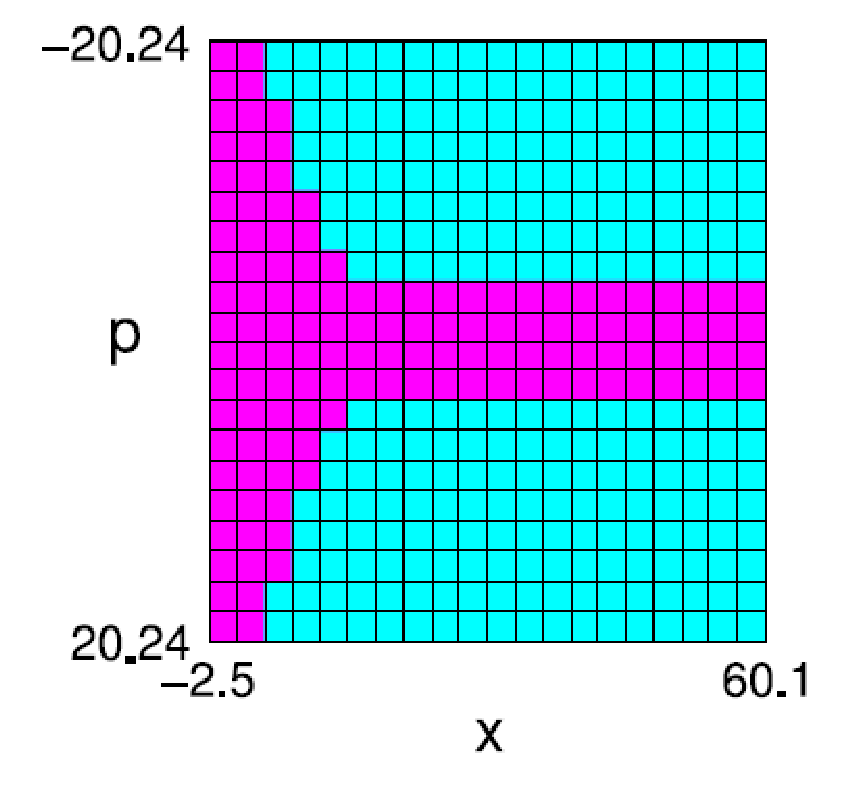
\includegraphics[width=2.0in]{Figures/morse_ps.eps}}
\subfigure{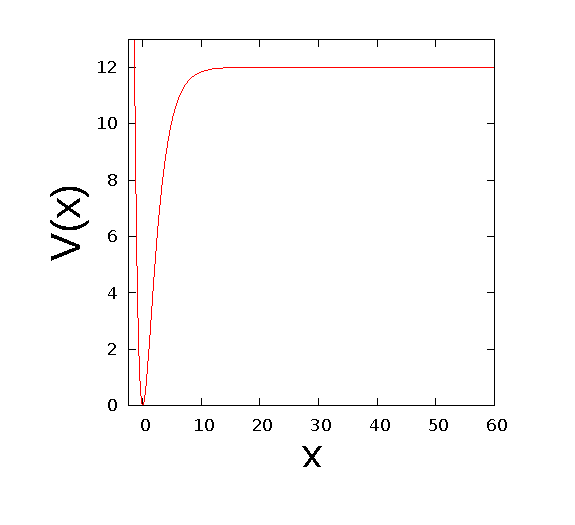
\includegraphics[width=2.1in]{Figures/morse_pl.eps}}}
\caption[The four (SP;1000) wavefunctions]{Left) The phase space grid of functions, $g_{i,j}$ are placed at the middle of squares with area $2\pi$. Right)Morse potential with parameters D=12,m=6,$\beta$=0.5} 
\label{fig.morse}
\end{figure}


The method employed by Ref.~\citenum{Halverson2012} is to form a basis using the Von Neumann lattice shown pictorially in Fig~\ref{fig.morse}. However, instead of each square occupying a area of size $2\pi\hbar$, you begin with a lattice that has square size $4\pi\hbar$.  In practice, you choose some $\Delta x=x_{n+1}-x_n$ that provides a suitable number of basis across the potential and then choose $\Delta p=p_{n+1}-p_n=2\pi \hbar/\Delta x$.  This ensures that you have one basis function per unit cell (of $\hbar$) in phasespace.  If Ref.~\citenum{Halverson2012} left the basis as this, it would be undercomplete and would not represent the wavefunctions well.  The reason to start with this half dense lattice is that the critically dense lattice (namely $\Delta x\Delta p=2\pi\hbar$) is not localized once the basis functions are orthogonalized\cite{Poirier2004}.

   Orthogonalization must occur in order to obtain eigenvalues, this is in general performed by Lowdin orthogonalization.  In this case, diagonalization of the overlap matrix $S_{i,j,i^{\prime},j^{\prime}}=\int g_{i,j}\left(x\right)g_{i^{\prime},j^{\prime}}$ is performed which results in the diagonal matrix $s$ and eigenvector matrix $T$.  The eigenvalues of the Hamiltonian can be found by diagonalizing $s^{1/2}T^{\dagger}HTs^{-1/2}$.  If you set up a vector $\vec{g}$ which has elements $g_{i,j}\left(x\right)$ then the vector of orthogonalized basis functions are $s^{-1/2}T\vec{g}$.  These functions turn out to only have inverse decay at critical density even though the individual $g_{i,j}\left(x\right)$ have exponential decay.  This was the motivation for starting with the half-dense representation.  In order to make the basis complete, Ref.~\citenum{Halverson2012} then uses the reciprocal lattice which is doubly dense (namely $\Delta x\Delta p=\pi\hbar$) and combines the two bases in a product fashion.  However, this results in overcompleteness so only the symmetric component of momentum is taken or $\left(G\left(-p\right)+G\left(p\right)\right)/\sqrt{2}$.  The resulting basis is
 \begin{equation}\label{eq.psdd}
 g_{i,j}=\left(\dfrac{4}{\pi}\right)^{1/4}\exp\left[-\dfrac{1}{2}\left(x-m\sqrt{\pi}\right)^2\right]\sin\left[n\sqrt{\pi}x-\dfrac{n\pi}{2}\left(2m+1\right)\right].
 \end{equation} 
 
 
 The second use of of Von Neumann lattice basis sets was proposed by Shimshovitz and Tannor in 2012\cite{Shimshovitz2012}.  This begins with the basis set of Eq.~(\ref{eq.wps1}) but instead of applying the Hamiltonian to Gaussians themselves, the initial Hamiltonian matrix is set up using the Fourier Grid Hamiltonian\cite{Tannor2007}.  The Fourier Grid Hamiltonian (FGH) basis is
 \begin{equation}\label{eq.four}
\phi_n \left(x\right) = \sum_{j=-N/2+1}^{N/2}\dfrac{1}{\sqrt{LN}} \exp\left[\dfrac{i2 \pi j}{L}\left(x-x_n\right)\right]
 \end{equation}
where $x_n$ are equally spaced points in the domain $[0,L]$.  This is commonly referred to as the Sinc discrete variable representation which has the same phase space as $N$ $g_{i,j}\left(x\right)$ basis functions with position space centres in $\left[0,L\right]$ and momentum space centres in $\left[-P,P\right]$. This correspondence between the FGH and Von Neumann bases is shown for the use of 9 sinc functions and a $3\time3$ grid in phasespace.  The sinc functions are centred on the grid on the bottom while the Von Neumann basis functions are centred in the middle of the squares.
\begin{figure}[!ht]
\begin{center}
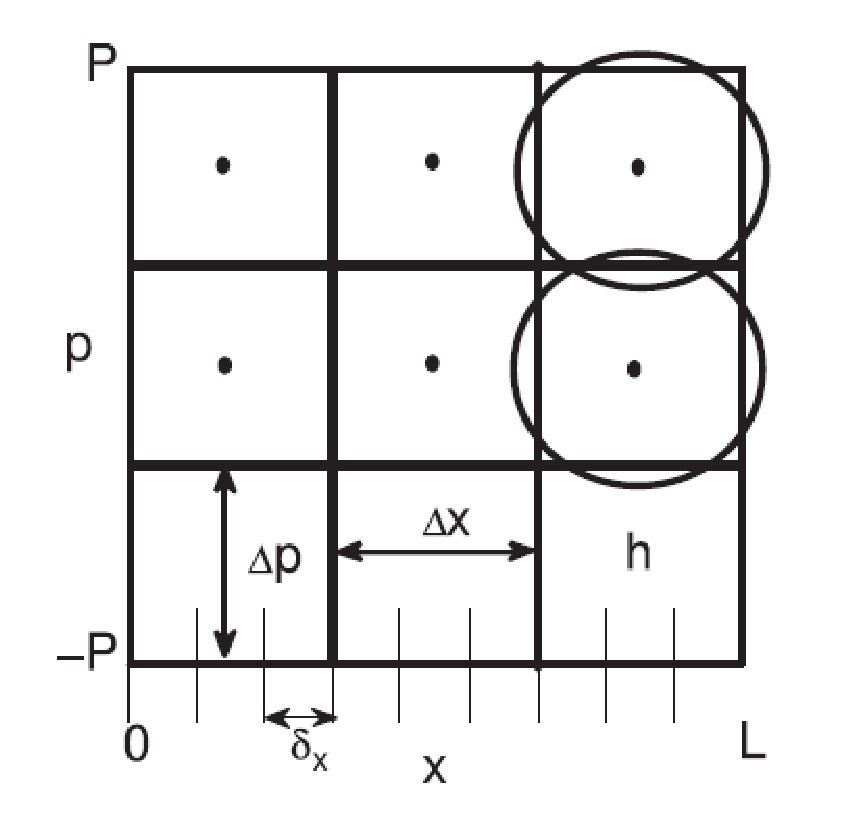
\includegraphics[scale=0.5]{shim.eps}
\caption{9 sinc and $3\time3$ Von Neumann basis functions. The sinc functions are centred on the dashed lines on the bottom while the Von Neumann basis functions are centred in the middle of the squares.}
\label{fig.r4}
\end{center}
\end{figure}

 From this, the basis functions are taken to be
\begin{equation}\label{eq.psfg}
\tilde{g}_{i,j}\left(x\right)=\sum_{n=1}^{N}\phi_n\left(x_n\right)g_{i,j}\left(x_n\right).
\end{equation}
If a $G$ matrix is defined with elements $G_{k,l}=g_{l}\left(x_k\right)$, where $l$ runs over all $i,j$ values, than Eq.~(\ref{eq.psfg}) can be rewritten as $\tilde{G}=\Phi G$. Since the $\Theta$ is diagonal, the matrix representation is
\begin{equation}\label{eq.psfg2}
H_{i,j,i^{\prime},j^{\prime}}U=.\sum_{m=1}^{N}\sum_{n=1}^{N}g_{i,j}\left(x_m\right)\left(\int \phi_m\left(x\right)H\phi_n\left(x\right)\right)g_{i^{\prime},j^{\prime}}\left(x_n\right)U=SU
\end{equation}
This basis turns out to not be conducive to pruning in that every basis function removed decreases the accuracy of the eigenvalues.  If you instead use basis functions $b_{k}\left((x\right)=\sum_{l=1}^N\tilde{g_{l}}\left(S^{-1}\right)_{l,k}$ then it results in the matrix representation
\begin{equation}\label{eq.psfg3}
H_{k,l}U=.\sum_{m=1}^{N}\sum_{n=1}^{N}b_{l}\left(x_m\right)\left(\int \phi_m\left(x\right)H\phi_n\left(x\right)\right)b_{k}\left(x_n\right)U=S^{-1}U
\end{equation}
which can be pruned without decreasing the accuracy.

\section{Applicability to OCS trimer}\label{sec.app}
In most cases where the above methods were implemented, the Watson 
Hamiltonian with a Taylor expansion of the PES around the (unique) equilibrium geometry was used.  This potential is of the form
\begin{equation}
V\left(\bf{x}\right)=\sum_{i=1}^N \omega_i x_i^2 + \sum_{i,j,k}c_{i,j,k}x_ix_jx_k+ \sum_{i,j,k,l}c_{i,j,k,l}x_ix_jx_kx_l,
\end{equation} 
where N is the number of degrees of freedom.  This Taylor expanded PES has a convenient form, such that only 1D integrals are required to obtain 
energies and has the proper boundary conditions for a Gaussian basis. 
That being said, as will be described later, the OCS dimer/trimer systems have many equilibrium geometries, so this expansion will not work.  There have been a couple cases where more general PESs were used.

In Ref.~\citenum{Garashchuk2001},  a DGB was applied to the $r_1$ and $r_2$ stretch coordinates for the vibration of the water molecule while the $\theta$ coordinate was represented with a Legendre DVR.  This calculation was performed by adding DGB functions of $r_1,r_2$ at each angle $\theta_a$ and checking to see if the $r_1,r_2$ portion of the Hamiltonian has it's eigenvalues converged to a certain precision.   Ref.~\citenum{Garashchuk2001} also calculated the vibrational energies of the Neon and Argon trimers.  The Hamiltonian used depended on the inter-atomic distances $r_1,r_2,r_3$ with the potential a sum of morse potentials of $r_1,r_2,r_3$.  These coordinates had to satisfy the triangle inequality $\left|r_1-r_3\right|\leq r_2 \leq r_1+r_2$ and allowed symmetry to easily be implemented.  For example, the $A_1$ symmetry is calculated by using a basis that is the normalized sum of the six permutations of $r_1,r_2,r_3$.


